\section{Lezione 4 - Operazioni aritmetiche con numeri approssimati}
Nelle lezioni precedenti abbiamo discusso una delle basi del calcolo numerico: il sistema floating-point di rappresentazione dei numeri reali nel calcolatore. \\
Il concetto cardine è quello di precisione di macchina, il massimo errore relativo di arrotondamento di un numero reale rappresentabile (ovvero non in overflow o underflow) con il reale-macchina ``più vicino".\\
In questa lezione inizieremo ad entrare nel cuore del calcolo numerico, trattando innanzitutto le operazioni aritmetiche nel sistema floating-point, cioè quale sia l'effetto degli errori sui dati, sul risultato dell'operazione.\\
L'analisi che faremo sarà però più generale e permetterà di studiare la risposta agli errori sui dati delle operazioni aritmetiche qualunque sia la fonte di errore (ad esempio errori di misura sperimentale).

\subsection{Operazione macchina}
Cominciamo col definire il concetto di OPERAZIONE-MACCHINA.\\
Sia $\bigstar$ un'operazione aritmetica sui reali, ovvero \[ \bigstar =
\begin{cases}
    \pm & \text{addizione, sottrazione} \\
    * & \text{moltiplicazione} \\
    / & \text{divisione}
\end{cases}
\]
Allora, dato un insieme di reali-macchina $\mathbb{F}(b, t, L, U)$ il modo in cui il processore realizza l'operazione tra due reali rappresentabili $x, y$ è 
\begin{center}
    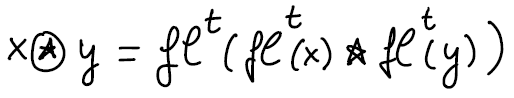
\includegraphics[scale=0.65]{foto/img11}
\end{center}
ovvero il modello è il seguente:
\begin{enumerate}
    \item i due reali vengono arrotondati
    \item viene fatta l'operazione tra gli arrotondamenti
    \item il risultato viene a sua volta arrotondato
\end{enumerate}
È importante osservare da subito che le operazioni-macchina nel sistema floating-point perdono varie proprietà delle operazioni aritmetiche teoriche. Ad esempio, mentre la proprietà commutativa di addizione e moltiplicazione resta valida, in generale non sono più valide la proprietà associativa e distributiva.\\
Facciamo un esempio in cui non vale la proprietà associativa della moltiplicazione,per problemi di overflow.
\begin{esempio} \end{esempio}
Consideriamo $\mathbb{F} = (10, 16, -307, 308)$ che come abbiamo visto corrisponde sostanzialmente all'interfaccia del Matlab. Siano
\[ a = 10^{200}\,,\,b = 10^{150}\,,\,c = 10^{-50} \]
in aritmetica reale \[ (a \times b) \times c = a \times (b \times c) = 10^{300} \]
Ma con le limitazioni date per gli esponenti \[(a \otimes b) \otimes c = \text{overflow}\]
perché  \[a \otimes b = 10^{350} \quad \text{e} \quad 350 >308\]
invece \[ a \otimes (b \otimes c) = 10^{200} \otimes 10^{100} = 10^{300} \]
Quindi \[ (a \otimes b) \otimes c \underbrace{\ne}_{\text{NO ASSOCIATIVA}} a \otimes (b \otimes c) = a \times b \times c \]
\newline \newline
Come vedremo più avanti, la proprietà associativa (e anche la distributiva) possono saltare anche per effetto degli errori di arrotondamento.\\
D'altra parte, c'è un'altra proprietà che non è più valida a causa dell'arrotondamento, l'unicità dell'elemento neutro dell'addizione.\\
Per capirlo, consideriamo di nuovo un sistema floating-point “virtuale” $\mathbb{F} = (10, 16, -307, 308)$ (qui in realtà conta essenzialmente il numero di cifre mantissa). Si ha 
\[ 1 \oplus 10^{-16} = 1\]
cioè $10^{-16}$ si comporta come 0 nell'addizione con 1, mentre 
\[ 1 \oplus 10^{-15} = 1 + 10^{-15}\]
Perché? Basta riflettere sul fatto che le cifre di mantissa sono 16, ma17cifra
\[ 1 + 10^{-16} = (0,100 \dotsc 0 \underbrace{1}_{17^\circ\text{ cifra}}) \cdot 10^1\]
viene arrotondato ad 1 perché la prima cifra trascurata è \[ 1 < \frac{b}{2} = 5 \]
Invece \[ 1 + 10^{-15} = (0,100 \dotsc 0 \underbrace{1}_{16^\circ\text{ cifra}}) \cdot 10^1\] 
e non c'è bisogno di alcun arrotondamento.
D'altra parte, si vede anche subito che $ 10^{-1} \oplus 10^{-16} = 10^{-1} + 10^{-16} $ cioè $10^{-16}$ non è l'elemento neutro per $10^{-1}$.\\
In questo contesto si può dare una seconda caratterizzazione della precisione di macchina (che non dimostriamo)
\[ \varepsilon_M = \min \{\mu \in \mathbb{F}^+ : 1 \oplus \mu > 1\} \]

\subsection{Risposta delle operazioni agli errori sui dati}
Passiamo alla questione chiave: la risposta delle operazioni agli errori \uline{sui dati}.\\
Possiamo osservare fin da subito che l'arrotondamento finale del risultato ha un errore che non può superare la precisione di macchina \[ \varepsilon_M = \frac{b^{1-t}}{2}\]
e quindi è ininfluente ai fini dell'analisi dell'effetto degli errori sui dati. \\
Invece l'errore chiave da stimare è l'errore \uline{relativo} 
\[ \varepsilon_{x \star y} = \frac{\lvert (x \star y) - (fl^t (x) \star fl^t (y)) \rvert}{\lvert (x \star y) \rvert} \]
(purché $(x \star y) \ne 0$) in funzione degli errori relativi sui dati
\[ \varepsilon_x = \frac{\lvert x - \Tilde{x} \rvert}{\lvert x \rvert}, \quad x \ne 0 \]
\[ \varepsilon_y = \frac{\lvert y - \Tilde{y} \rvert}{\lvert y \rvert}, \quad y \ne 0 \]
Più in generale, dati due numeri reali $x, y \ne 0$ e due loro approssimazioni $\Tilde{x} \approx x\,,\, \Tilde{y} \approx y$ (dove supponiamo di conoscere o meglio di saper stimare gli errori relativi $ \varepsilon_x = \frac{\lvert x - \Tilde{x} \rvert}{\lvert x \rvert}$ e $ \varepsilon_y = \frac{\lvert y - \Tilde{y} \rvert}{\lvert y \rvert}$ ) andremo a stimare l'errore relativo sul risultato dell'operazione $\star$, commesso utilizzando i dati approssimati invece dei dati esatti, cioè
\[ \varepsilon_{x \star y} = \frac{\lvert (x \star y) - (\Tilde{x} \star \Tilde{y}) \rvert}{\lvert (x \star y) \rvert}, \quad x \star y \ne 0 \]
in funzione di $\varepsilon_x$, $\varepsilon_y$ (nel caso delle operazioni-macchina si ha $\Tilde{x} = fl^t(x)$, $\Tilde{y} = fl^t(y)$, $\varepsilon_x$, $\varepsilon_y \le \varepsilon_M$).
Diremo STABILE un'operazione aritmetica per cui l'errore sul risultato ha lo stesso ordine di grandezza dell'errore (massimo) sui dati.

\subsubsection{Moltiplicazione}
Iniziamo con la MOLTIPLICAZIONE (indicheremo il prodotto con la notazione standard $\times \, y$, sapendo che nei linguaggi di calcolo il simbolo delle moltiplicazione è *).
\[ \varepsilon_{xy} = \frac{\lvert \, xy - \Tilde{x}\Tilde{y} \, \rvert}{\lvert \, xy \, \rvert}, \quad x , y \ne 0 \]
Usiamo la stessa tecnica che si usa per dimostrare che il limite del prodotto di due successioni o funzioni è il prodotto dei limiti, aggiungendo e togliendo a numeratore ad esempio $\Tilde{x}y$
\[\begin{split}
    \varepsilon_{xy} & = \frac{\lvert \, xy - \Tilde{x}y + \Tilde{x}y - \Tilde{x}\Tilde{y} \, \rvert}{\lvert \, y \, \rvert} \\
    & = \frac{\lvert \, \overbrace{y(x - \Tilde{x})}^{=\,a} + \overbrace{x(y - \Tilde{y})}^{=\,b} \, \rvert}{\lvert\, xy \, \rvert} \\
    & \le \frac{\lvert \, y(x - \Tilde{x}) + x(y - \Tilde{y}) \, \rvert}{\lvert \, xy \, \rvert} \quad \quad (\bigstar) 
\end{split}\]
dove abbiamo utilizzato la DISUGUAGLIANZA TRIANGOLARE che è uno strumento chiave per fare stime.\\
Dati $a, b \in \mathbb{R}$
\[ \lvert \lvert \, a \, \rvert - \lvert \, b \, \rvert \rvert \le \lvert \, a + b \, \rvert \le \lvert \, a \, \rvert + \lvert \, b \, \rvert\] 
Quindi da $(\bigstar)$ otteniamo (ricordando che il modulo del prodotto è il prodotto dei moduli)
\[ \varepsilon_{xy} \le \frac{\lvert \,y\, \rvert \lvert \,x - \Tilde{x}\, \rvert}{\lvert \,xy\, \rvert} + \frac{\lvert \,\Tilde{x}\, \rvert \lvert \,y - \Tilde{y}\, \rvert}{\lvert \,xy\, \rvert} = \varepsilon_x + \frac{\lvert \,\Tilde{x}\, \rvert}{\lvert \,x\, \rvert} \varepsilon_y\]
Questo perché $\frac{\lvert \,x - \Tilde{x}\, \rvert}{\lvert \,x\, \rvert} = \varepsilon_x$ e $\frac{\lvert \,y - \Tilde{y}\, \rvert}{\lvert \,y\, \rvert} = \varepsilon_y$.\\
Ora, siccome $\Tilde{x} \approx x$, possiamo dire almeno qualitativamente che $\frac{\lvert \,\Tilde{x}\, \rvert}{\lvert \,x\, \rvert} \approx 1$ e quindi 
\[ \varepsilon_{xy} \le \varepsilon_x + \frac{\lvert \,\Tilde{x}\, \rvert}{\lvert \,x\, \rvert} \varepsilon_y \approx \varepsilon_x + \varepsilon_y \]
cioè che l'operazione di moltiplicazione è STABILE (l'errore relativo sul risultato è maggiorato da una quantità che è dell'ordine dell'errore sui dati).\\
Per esprimere questo fatto possiamo usare la notazione \[\varepsilon_{xy} \lesssim \varepsilon_x + \varepsilon_y \]
dove $\lesssim$ non è una disuguaglianza esatta ma va intesa nel senso indicato sopra. \\
In realtà, possiamo dare anche una \uline{stima} quantitativa osservando che per la disuguaglianza triangolare 
\[ \frac{\lvert \,\Tilde{x}\, \rvert}{\lvert \,x\, \rvert} = \frac{\lvert \, \overbrace{x}^{=\,a} + \overbrace{\Tilde{x} - x}^{=\,b} \, \rvert}{\lvert\, x \, \rvert} \le \frac{\lvert \, x \, \rvert + \lvert \,\Tilde{x} - x\, \rvert}{\lvert\, x \, \rvert} = 1 + \varepsilon_x\]
e quindi \[ \varepsilon_{xy} \le \varepsilon_x + (1 + \varepsilon_x)\,\varepsilon_y\]
Nel caso della moltiplicazione-macchina in precisione doppia $\varepsilon_x \le \varepsilon_M \approx 10^{-16}$ e quindi $1 + \varepsilon_x$ è vicinissimo ad 1.\\
Ma anche con $\varepsilon_x \approx 10^{-1}$ (ad esempio un errore di misura del $10\%$, che è un errore sperimentale grande) avremmo $1 + \varepsilon_x \approx 1,1$ e quindi la sostanza della stabilità non cambia.

\subsubsection{Divisione}
Passiamo ora alla DIVISIONE: siccome la divisione $\frac{x}{y}, \, y \ne 0$ è la moltiplicazione per il reciproco, $\frac{x}{y} = x \cdot \frac{1}{y}$, ci basta analizzare la stabilità dell'operazione di reciproco
\[ \varepsilon_{\frac{1}{y}} = \frac{\abs*{\,\frac{1}{y} - \frac{1}{\Tilde{y}}\,} }{\abs*{\,\frac{1}{y}\,}} = \frac{\frac{\abs*{\,\Tilde{y} - y\,}}{\abs*{\,\Tilde{y}y\,}}}{\abs*{\,\frac{1}{y}\,}} = \frac{\abs*{\,\Tilde{y} - y\,}}{\abs*{\,y\,}} \cdot \frac{\abs*{\,y\,}}{\abs*{\,\Tilde{y}\,}} \approx \varepsilon_y \qquad \Bigl( \text{questo perché } \frac{\abs*{\,\Tilde{y} - y\,}}{\abs*{\,y\,}} = \varepsilon_y . \Bigr)\]
con l'ipotesi qualitativa che $\abs{y} \approx \abs{\Tilde{y}}$ e quindi $\frac{\abs*{\,y\,}}{\abs*{\,\Tilde{y}\,}} \approx 1$ ne deduciamo che anche che la DIVISIONE è un'operazione STABILE, perché il reciproco è stabile e la moltiplicazione è stabile.\\
Anche in questo caso possiamo però quantificare, stimando meglio $\frac{\abs*{\,y\,}}{\abs*{\,\Tilde{y}\,}}$.\\ 
Assumiamo $\varepsilon_y = \frac{\abs*{\,y - \Tilde{y}\,}}{\abs*{\,y\,}} < 1$ (cioè che l'errore relativo sia minore di 1, il che vuol dire $< 100\%$, che sarà vero in tutte le situazioni “ragionevoli”, visto che tipicamente l'errore sarà molto più piccolo di 1), allora 
\[ \abs{\,\Tilde{y}\,} = \abs{\,y + \Tilde{y} - y\,} = \abs{y}\abs*{\,1 + \frac{(\Tilde{y} - y)}{y}\,}\]
usando la stima da sotto nella disuguaglianza triangolare 
\[\abs{\, a + b\,} \ge \abs{\,\abs{\,a\,} - \abs{\,b\,}\,}\]
$a = 1$ e $b = \frac{(\Tilde{y} - y)}{y}$
\[\abs*{\,1 + \frac{(\Tilde{y} - y)}{y}\,} \ge \abs*{\,1 - \frac{\abs*{\,\Tilde{y} - y\,}}{\abs{\,y\,}}\,} = \abs*{\,1 - \varepsilon_y\,} = 1 - \varepsilon_y \qquad \Bigl( \text{perché } \varepsilon_y < 1 \Bigr)\]
da cui si ottiene 
\[\abs{\,\Tilde{y}\,} \ge \abs{\,y\,}(1 - \varepsilon_y)\]
e quindi
\[\frac{\abs*{\,y\,}}{\abs*{\,\Tilde{y}\,}} \le \frac{\abs*{\,y\,}}{\abs{\,y\,}(1 - \varepsilon_y)} = \frac{1 + \varepsilon_y}{(1 + \varepsilon_y)(1 - \varepsilon_y)} = \frac{1 + \varepsilon_y}{1 - \varepsilon_y^2} \approx 1 + \varepsilon_y\]
perché $\varepsilon_y^2 \ll \varepsilon_y < 1$ (per la prima volta usiamo qui il simbolo ``$\ll$" molto minore) \\
Alla fine otteniamo
\[\varepsilon_{\frac{1}{y}} = \varepsilon_y\,\frac{\abs{\,y\,}}{\abs{\,\Tilde{y}\,}} \lesssim \varepsilon_y (1 + \varepsilon_y) \approx \varepsilon_y\]
cioè abbiamo quantificato in modo più preciso la stima qualitativa 
\[\frac{\abs*{\,y\,}}{\abs*{\,\Tilde{y}\,}} \approx 1\]
Riassumendo, moltiplicazione e divisione sono operazioni stabili visto che 
\[\varepsilon_{xy} \lesssim \varepsilon_x + \varepsilon_y\]
\[\varepsilon_{\frac{x}{y}} \lesssim \varepsilon_x + \varepsilon_{\frac{1}{y}} \lesssim  \varepsilon_x + \varepsilon_y\]

\subsubsection{Addizione e sottrazione}
Restano da analizzare addizione e sottrazione. Ma quando parliamo di addizione e quando di sottrazione, tenendo presente che i numeri possono avere segno qualsiasi?\\
Quello che faremo è analizzare la risposta agli errori sui dati della \uline{somma algebrica} $x + y$, ma tale somma (non importa il segno del risultato, è effettivamente un'\uline{addizione} se $x$ e $y$ hanno lo \uline{stesso segno}, è invece una \uline{sottrazione} se hanno \uline{segni diversi})
\[\begin{split}
    \varepsilon_{x+y} & = \frac{\abs*{\,(x + y) - (\Tilde{x} + \Tilde{y})\,}}{\abs*{\,x + y\,}} \,, \quad x + y \ne 0 \\
    & = \frac{\abs*{\,x - \Tilde{x} + y - \Tilde{y}\,}}{\abs*{\,x + y\,}} \,, \quad a = x - \Tilde{x} \text{ e } b = y - \Tilde{y} \\
    & \le \frac{\abs*{\,x - \Tilde{x}\,}}{\abs*{\,x + y\,}} + \frac{\abs*{\,y - \Tilde{y}\,}}{\abs*{\,x + y\,}} \,, \quad \text{DISUGUAGLIANZA TRIANGOLARE} \\
    & = \frac{\abs*{\,x\,}}{\abs*{\,x + y\,}} \cdot \frac{\abs*{\,x - \Tilde{x}\,}}{\abs*{\,x\,}} + \frac{\abs*{\,y\,}}{\abs*{\,x + y\,}} \cdot \frac{\abs*{\,y - \Tilde{y}\,}}{\abs*{\,y\,}} \\
    & = w_1 \varepsilon_x + w_2 \varepsilon_y
\end{split}\]
dove $w_1 = \frac{\abs*{\,x\,}}{\abs*{\,x + y\,}}$, $w_2 = \frac{\abs*{\,y\,}}{\abs*{\,x + y\,}}$ .\\
Abbiamo quindi maggiorato $\varepsilon_{x+y}$ con una \uline{somma pesata} degli errori sui dati, con pesi $w_1$ e $w_2$.\\
Si noti che questi pesi dipendono da $x$ e da $y$, ma \uline{non dipendono} dagli errori.\\
In realtà anche con la moltiplicazione e la divisione siamo arrivati in sostanza a una stima del tipo
\[\varepsilon_{x \bigstar y} \le w_1 \varepsilon_x + w_2 \varepsilon_y\]
dove $w_1, w_2 \approx 1$. \\
Vedremo ora che questa è anche la situazione con l'addizione, mentre le cose possono cambiare radicalmente con la sottrazione \\
\[\text{ADDIZIONE} (sign(x) = sign(y))\]
in questo caso $\abs{\,x + y\,} \ge \abs{\,x\,}\,,\,\abs{\,y\,}$ si pensi per semplicità al caso $x,y > 0$, è chiaro che $x + y > x$ e $x + y > y$) \\
Quindi
\[w_1 = \frac{\abs*{\,x\,}}{\abs*{\,x + y\,}} \le 1 \quad , \quad w_2 = \frac{\abs*{\,y\,}}{\abs*{\,x + y\,}} \le 1\]
cioè \[\varepsilon_{x+y} \le \varepsilon_x + \varepsilon_y\]
ovvero l'addizione è STABILE (l'errore relativo sul risultato è maggiorato da una quantità che è dell'ordine degli errori sui dati)
\[\text{SOTTRAZIONE} (sign(x) \ne sign(y))\]
in questo caso $\abs{\,x + y\,} < \abs{\,x\,}$ oppure $\abs{\,x + y\,} < \abs{\,y\,}$ quindi $\max \{w1 , w2\} > 1$. \\
Questo ci dice che la sottrazione può far perdere precisione rispetto agli errori sui dati, ma quanta? In effetti può succedere che $\abs{\,x\,}$ e $\abs{\,y\,}$ siano molto vicini in termini relativi cioè che $\abs{\,x + y\,} \ll \abs{\,x\,}\,,\,\abs{\,y\,}$ \\
In queste situazioni $w_1\,,\,w_2 \gg 1$ e la sottrazione diventa INSTABILE.\\
Si noti che $w_1$ e $w_2$ possono essere arbitrariamente grandi, dipende dai dati.\\
È importante osservare che si tratta di un problema di “vicinanza” relativa, non assoluta, tra le due quantità che vengono sottratte, cioè i casi instabili non sono quelli in cui $\abs{\,x + y\,}$ è “piccolo”, ma quelli in cui è piccolo rispetto a $\abs{\,x\,}\,,\,\abs{\,y\,}$.
Ad esempio sono analoghi: 
\begin{center}
    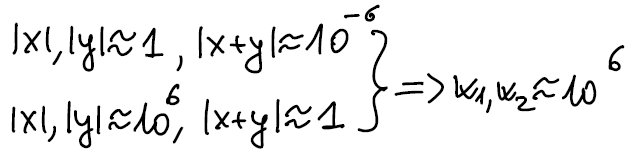
\includegraphics[scale=0.65]{foto/img12}
\end{center}
Detto a parole, due numeri dell'ordine delle unità che distano di qualche milionesimo, sono altrettante vicini in termini relativi di due numeri dell'ordine del milione che distano di qualche unità.

In entrambi i casi i pesi $w_1$, $w_2$ sono fattori di amplificazione dell'errore dell'ordine di $10^6$.\\
Possiamo sintetizzare che la SOTTRAZIONE è \uline{potenzialmente} (non sempre) \uline{INSTABILE}.\\
Infatti se $\abs{\,x\,}$ e $\abs{\,y\,}$ sono distanti in termini relativi, la sottrazione perderà poca precisione.\\
Se invece sono vicini perderà molta precisione, tanta più quanto più sono vicini.\\
Questo fenomeno (che si chiama anche “cancellazione numerica”) è il primo e importante esempio di possibile instabilità di un algoritmo (in questo caso la semplice operazione di sottrazione tra numeri approssimati).\\
È un fenomeno che studieremo meglio con degli esempi e che si può fronteggiare in 2 modi:
\begin{enumerate}
    \item cercare di riscrivere le espressioni e gli algoritmi in modo da evitare sottrazioni instabili (lo vedremo ad esempio con la formula risolutiva per le equazioni di $2^\circ$ grado)
    \item aumentando la precisione (cioè diminuendo l'errore sui dati) in funzione della grandezza di $w_1$ e $w_2$
\end{enumerate}
In campo sperimentale, questo significa aumentare la precisione dello strumento di misura. Nel caso dell'arrotondamento, questo significa andare in un sistema floating-point a precisione estesa, se ad esempio $w_1$ e $w_2$ sono così grandi da mettere in crisi un sistema a precisione doppia. Si tenga conto che come vedremo $w_1$ e $w_2$ possono essere arbitrariamente grandi e quindi far perdere completamente di significato al risultato quando $w_1, w_2 > \frac{1}{\varepsilon_M}$.\\
Come già osservato però, usare precisioni estese può avere un costo computazionale molto elevato in termini di tempo di calcolo e di occupazione di memorie.\\
Nella prossima lezione faremo vari esempi di perdita di precisione dovuta ad una sottrazione e di stabilizzazione (quando possibile) dell'algoritmo di calcolo evitando tale sottrazione.\\
Per fissare le idee, facciamo però subito un esempio significativo: 
\begin{esempio}\end{esempio}
Consideriamo la funzione
\[f(x) = \frac{((1 + x) - 1)}{x}, \quad x \ne 0\]
è evidente che $f(x) = 1$ (è la funzione costante 1) però, calcolando in Matlab $f(10^{-15})$ si ottiene $f(10^{-15}) = 1.11\dotsc$ cioè l'errore relativo sul risultato è $>11\%$ (un errore enorme rispetto all'arrotondamento che non supera $\varepsilon_M \approx 10^{-16}$)\\
Vedremo che la spiegazione sta nella sottrazione a numeratore, visto che $1+10^{-15}$ è vicinissimo ad 1.\\
Invece $f(2^{-50}) = 1$, pur essendo $2^{-50} \approx 10^{-15}$ perché?\\
Tratteremo entrambi i casi nella prossima lezione.
\newpage